\chapter{Experiments}
\label{chapter:experiments}

\section{Full Lap Planning}

In this experiment we test the Hybrid A* and \gls{SEHS} algorithms as we described them in Section~\ref{sec:trajectory_planning_algorithms} on several different circuit maps. For each circuit, the algorithms should find a near time-optimal trajectory from a starting position through a series of waypoints until the last waypoint of the circuit is reached. We then compare the quality of the solutions, how much of the state space the algorithm had to explore before it found the solution, and how long it took to calculate the result on the testing computer.

\subsection{Test Setup}

The parameters of the vehicle chassis and the vehicle model we used are equal to the properties of our experimental vehicle as stated in Table~\ref{table:dimensions} and derived in Section~\ref{sec:actuators_model}.

Both Hybrid A* and \gls*{SEHS} require specification of state space and time discretization parameters. We found that both algorithms performed well with time step $\Delta t=\SI{0.04}{\second}$ (\SI{25}{\hertz}), the heading angle values divided into \num{28} sectors of a circle, and the range of possible values of motor \gls*{RPM} divided into \num{10} sub-ranges. Additionally, the Hybrid A* algorithm splits the $x$ and $y$ coordinates were split into squares with side lengths of $4r$, where $r$ is the radius of the vehicle. The SEHS algorithm discretizes the $xy$ plane by finding a path of circles in the Space Exploration step. We require the radii of the circles to be between $r$ a $5r$. The actions available to the planner were a cross product of 6 throttle levels (\num{-0.25} - \num{1}) and 21 steering angles (\num{-1} - \num{1}).

Circuits are represented by an occupancy grid bitmap with a resolution of \SI{0.05}{\meter} per grid cell. For each circuit, we first perform track segmentation, as described in Section~\ref{sec:track_segmentation}, to detect corners which we use as waypoints. We also perform the Space Exploration step of the SEHS algorithm. We then let both algorithms find the near time-optimal trajectory from the initial configuration defined for each circuit to the last waypoint. We measure the number of search nodes the algorithm opens during search, the number of search nodes which are expanded, and also the time it takes to find the solution on a testing computer. Because both of the algorithms are deterministic, they always find the same solution for the same problem and they always open and expand the same number of search nodes. The execution times differ slightly and so we repeat the measurement 20 times and calculate the average execution time.

These values were not selected at random, but rather by evaluating the performance and the quality of the solutions for different values. The selected parameters yielded good quality results while being reasonably fast.

We used a desktop computer with an AMD Ryzen 7 3700X CPU running at the base clock of \SI{3.6}{\giga\hertz} and \num{32}GB of DDR4 RAM at the base clock of \SI{3200}{\mega\hertz}. The source code was written in C++17 and compiled using GCC 9.2 with the \texttt{-O3} and \texttt{-ffast-math} optimization flags.

\subsection{Results}

The results of our experiments are shown in Figure~\ref{fig:porto},~\ref{fig:tornado},~\ref{fig:simple},~\ref{fig:u}, and~\ref{fig:zurich}.

Each figure shows the trajectory as a curve from the initial configuration (marked with a green arrow) to a final configuration which passes the last waypoint (marked with a red waypoint). The black stars along the trajectory are a visual aid which marks the position of the vehicle every 1 second. The waypoints found by the track segmentation algorithm are marked as blue circles.

The curve which represents the trajectory of the vehicle has a color ranging from red to green. The color corresponds to the speed of the vehicle at the given position. The segments where the vehicle moves slowly is shown in red and the faster the car is moving the closer the color is to bright green.

The trajectory is plotted over a map of the circuit with white parts showing the road and gray parts the boundaries of the track. As we mentioned earlier, the occupancy grids for the circuits all have resolution of \SI{0.05}{\meter}. Every \num{20} grid cells correspond to \SI{1}{\meter} in real world. Therefore for example the circuit in Figure~\ref{fig:zurich} represents an area of \SI{25}{\meter} $\times$ \SI{25}{\meter}.

Each trajectory is accompanied by three charts, showing the control inputs for the vehicle, the normalized state of the actuators, and the speed profile of the trajectory.

\todo[inline]{Add commentary for the results.}

The trajectories found by the planning algorithms are very ambitious. The algorithm utilizes the kinematic model and so it assumes that the car will be able to make very sharp turns at very high speeds. It is highly unlikely that any vehicle would be able to exactly follow the planned trajectories.

It is interesting to observe that even though the \gls*{SEHS} algorithm usually opens and expands fewer search graph nodes, the total computation time can be higher than the computation time of Hybrid A*. There is significant overhead determining which circle is closest to a given point. We tried improving this using \texttt{kd}-trees for faster nearest neighbor search, but that in turn slowed down the computation when compared to simple linear search.


\begin{figure}[!tbp]%
	\centering

	\begin{subfigure}[t]{\textwidth}
		\begin{subfigure}[t]{0.45\textwidth}
			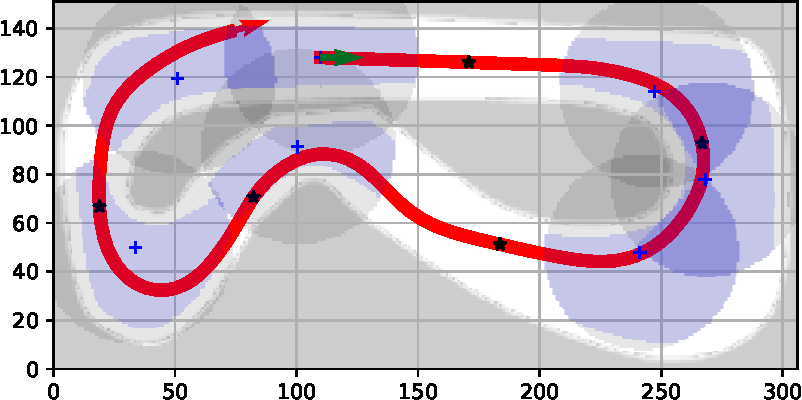
\includegraphics[width=\textwidth]{../img/experiments/porto-hybrid_astar-trajectory}
		\end{subfigure}
		\hfill
		\begin{subfigure}[t]{0.45\textwidth}
			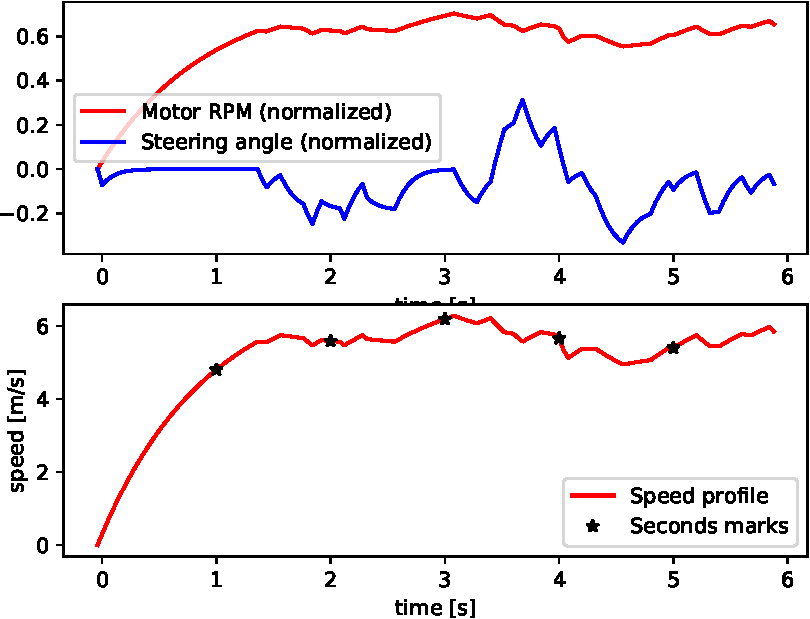
\includegraphics[width=\textwidth]{../img/experiments/porto-hybrid_astar-actuators}
		\end{subfigure}
		\caption{Solution found by Hybrid A* in \SI{192.30}{\milli\second}}
		\label{fig:solution_porto-hybrid_astar}	
	\end{subfigure}
	
	\vspace{0.75cm}
	
	\begin{subfigure}[t]{\textwidth}
		\begin{subfigure}[t]{0.45\textwidth}
			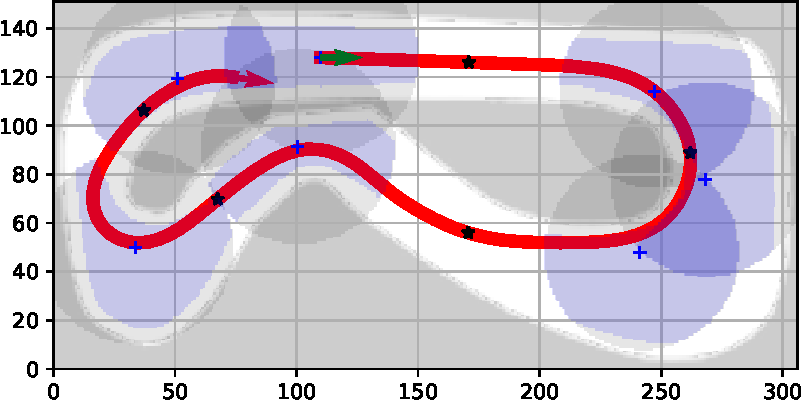
\includegraphics[width=\textwidth]{../img/experiments/porto-sehs-trajectory}
		\end{subfigure}
		\hfill
		\begin{subfigure}[t]{0.45\textwidth}
			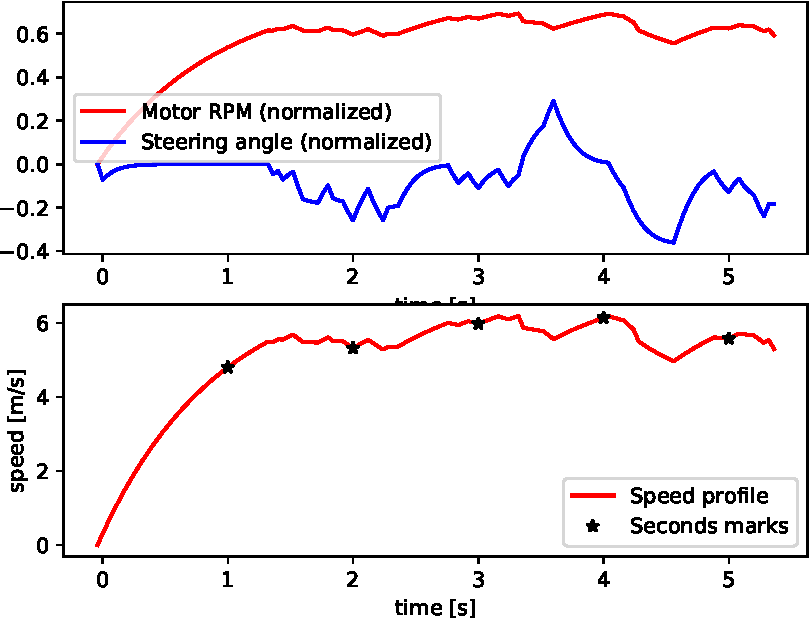
\includegraphics[width=\textwidth]{../img/experiments/porto-sehs-actuators}
		\end{subfigure}
		\caption{Solution found by SEHS in \SI{253.60}{\milli\second}}
		\label{fig:solution_porto-sehs}
	\end{subfigure}

	\vspace{0.75cm}

	\begin{subfigure}[t]{\textwidth}
		\centering
		\begin{tabular}{r r r r r r r r}%
			\toprule
			Actions & Grid cell size & RPM levels & Heading angle sectors & Opened & Expanded & Search time & Distance & Lap time \\	
			\midrule
			\num{44} & \num{1.80} & \num{20} & \num{18} & \bftab \num{67301} & \bftab \SI{192.30}{\milli\second} & \SI{39.94}{\meter} & \SI{13.64}{\second} \\
			\num{248} & \num{1.44} & \num{20} & \num{36} & \num{838926} & \SI{2544.00}{\milli\second} & \SI{36.99}{\meter} & \bftab \SI{12.28}{\second} \\
			\bottomrule
		\end{tabular}
		\caption{Hybrid A* found both a trajectory in the least amout of time and also a trajectory with the best lap time.}
		\label{table:porto-hybrid_astar}
	\end{subfigure}
	
	\begin{subfigure}[t]{\textwidth}
		\centering
		\begin{tabular}{r r r r r r r r r}%
			\toprule
			Actions & Circles & RPM levels & Heading angle sectors & Opened & Expanded & Search time & Distance & Lap time \\			
			\midrule
			\num{44} & \num{71} & \num{20} & \num{18} & \num{80763} & \SI{253.60}{\milli\second} & \SI{39.62}{\meter} & \SI{13.16}{\second} \\
			\num{84} & \num{71} & \num{80} & \num{36} & \num{1054427} & \SI{2171.60}{\milli\second} & \SI{37.50}{\meter} & \SI{12.48}{\second} \\
			\bottomrule
		\end{tabular}
		\caption{SEHS could not find a solution faster nor could it find a better solution than Hybrid A* with any of the tested combination of parameters.}
		\label{table:porto-sehs}
	\end{subfigure}
	
	\vspace{0.75cm}
	
	\caption{Circuit ``Porto''}
	\label{fig:porto}
\end{figure}

\begin{figure}[!tbp]%
	\centering
	
	\begin{subfigure}[t]{\textwidth}
		\begin{subfigure}[t]{0.45\textwidth}
			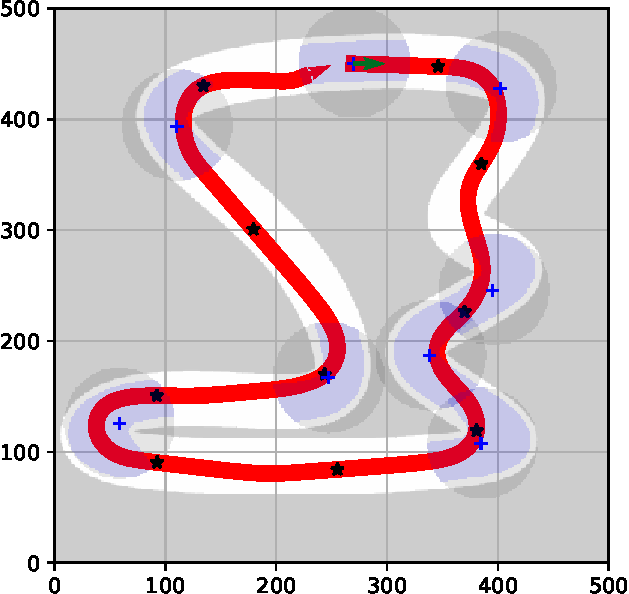
\includegraphics[width=\textwidth]{../img/experiments/tornado-hybrid_astar-trajectory}
		\end{subfigure}
		\hfill
		\begin{subfigure}[t]{0.45\textwidth}
			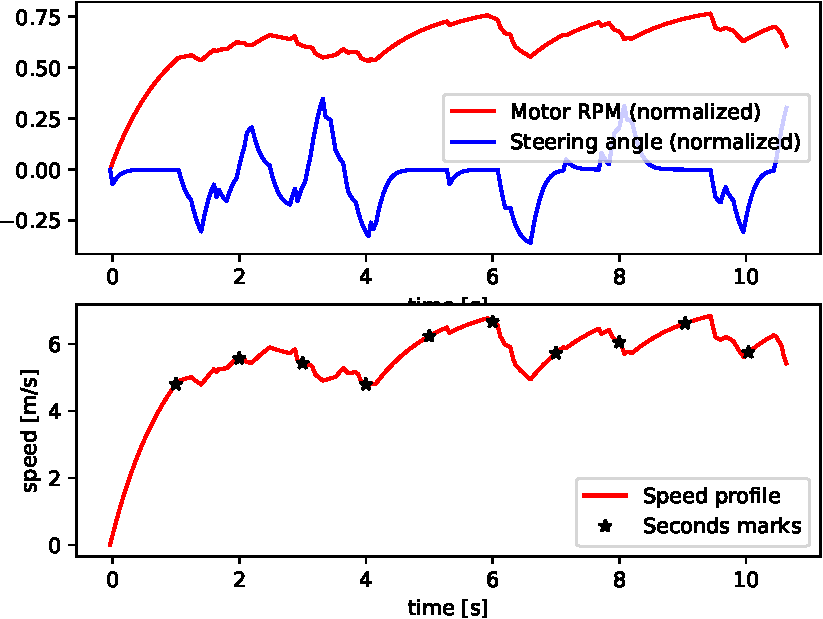
\includegraphics[width=\textwidth]{../img/experiments/tornado-hybrid_astar-actuators}
		\end{subfigure}
		\caption{Solution found by Hybrid A* in \SI{494.50}{\milli\second}}
		\label{fig:solution_tornado-hybrid_astar}	
	\end{subfigure}
	
	\vspace{0.75cm}
	
	\begin{subfigure}[t]{\textwidth}
		\begin{subfigure}[t]{0.45\textwidth}
			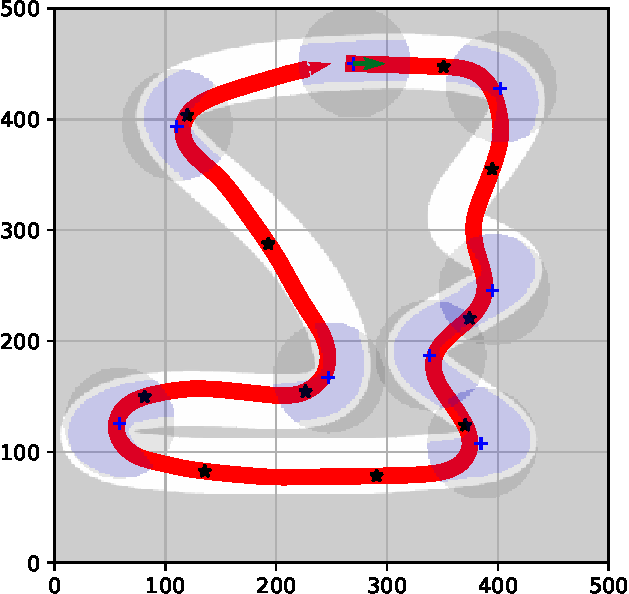
\includegraphics[width=\textwidth]{../img/experiments/tornado-sehs-trajectory}
		\end{subfigure}
		\hfill
		\begin{subfigure}[t]{0.45\textwidth}
			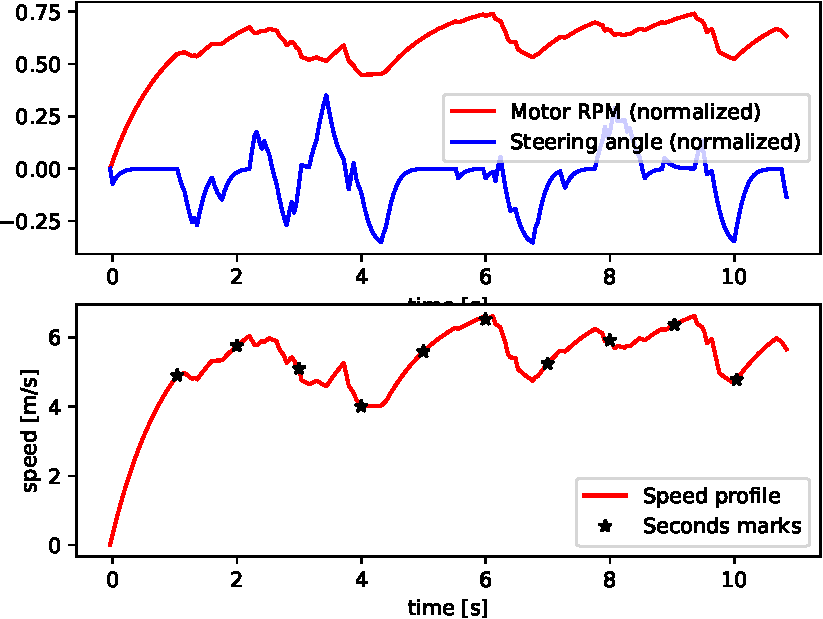
\includegraphics[width=\textwidth]{../img/experiments/tornado-sehs-actuators}
		\end{subfigure}
		\caption{Solution found by SEHS in \SI{551.30}{\milli\second}}
		\label{fig:solution_tornado-sehs}
	\end{subfigure}
	
	\vspace{0.75cm}
	
	\begin{subfigure}[t]{\textwidth}
		\centering
		\begin{tabular}{r r r r r r r r}%
            \toprule
                Actions & Grid cell size & RPM levels & Heading angle sectors & Opened & Expanded & Search time & Distance & Lap time \\
            \midrule
                \num{44} & \num{1.44} & \num{20} & \num{18} & \num{177778} & \bftab \SI{494.50}{\milli\second} & \SI{85.22}{\meter} & \SI{28.64}{\second} \\
                \num{84} & \num{1.44} & \num{80} & \num{52} & \num{3464766} & \SI{6611.70}{\milli\second} & \SI{84.96}{\meter} & \bftab \SI{26.24}{\second} \\
			\bottomrule
		\end{tabular}
		\caption{Hybrid A*: }
		\label{table:tornado-hybrid_astar}
    \end{subfigure}
    
    \begin{subfigure}[t]{\textwidth}
		\centering
		\begin{tabular}{r r r r r r r r}%
            \toprule
                Actions & Circles & RPM levels & Heading angle sectors & Opened & Expanded & Search time & Distance & Lap time \\
            \midrule
                \num{44} & \num{126} & \num{20} & \num{18} & \bftab \num{144864} & \SI{551.30}{\milli\second} & \SI{87.37}{\meter} & \SI{28.08}{\second} \\
                \num{84} & \num{126} & \num{80} & \num{52} & \num{2827948} & \SI{6397.60}{\milli\second} & \SI{84.68}{\meter} & \SI{26.84}{\second} \\
			\bottomrule
		\end{tabular}
		\caption{SEHS: }
		\label{table:tornado-sehs}
	\end{subfigure}
	
	\vspace{0.75cm}
	
	\caption{Circuit ``Tornado''}
	\label{fig:tornado}
\end{figure}

\begin{figure}[!tbp]%
	\centering

	\begin{subfigure}[t]{\textwidth}
		\begin{subfigure}[t]{0.45\textwidth}
			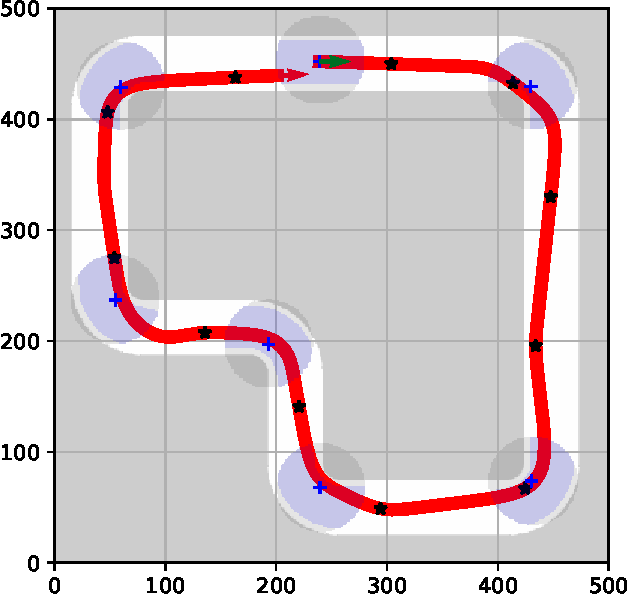
\includegraphics[width=\textwidth]{../img/experiments/simple-hybrid_astar-trajectory}
		\end{subfigure}
		\hfill
		\begin{subfigure}[t]{0.45\textwidth}
			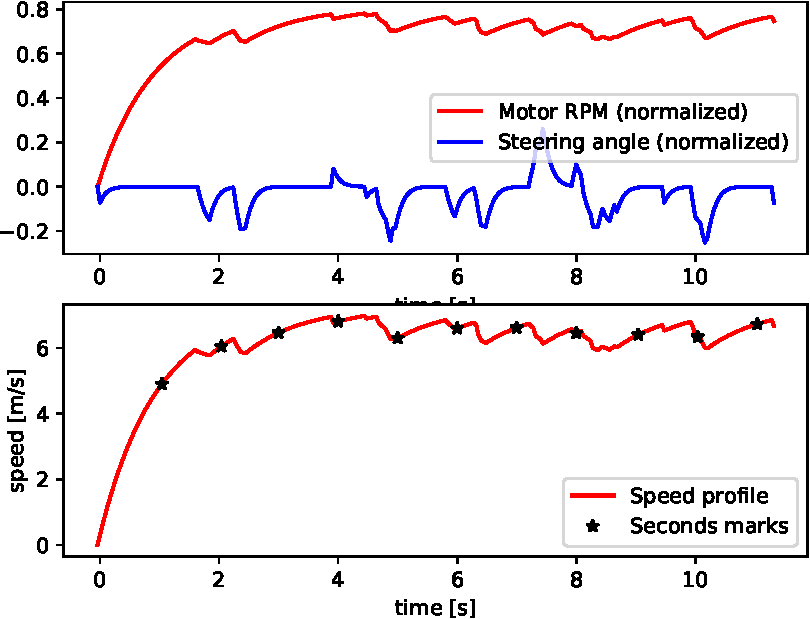
\includegraphics[width=\textwidth]{../img/experiments/simple-hybrid_astar-actuators}
		\end{subfigure}
		\caption{Solution found by Hybrid A* in \SI{236.20}{\milli\second}}
		\label{fig:simple-hybrid_astar}
	\end{subfigure}

	\vspace{0.75cm}
	
	\begin{subfigure}[t]{\textwidth}
		\begin{subfigure}[t]{0.45\textwidth}
			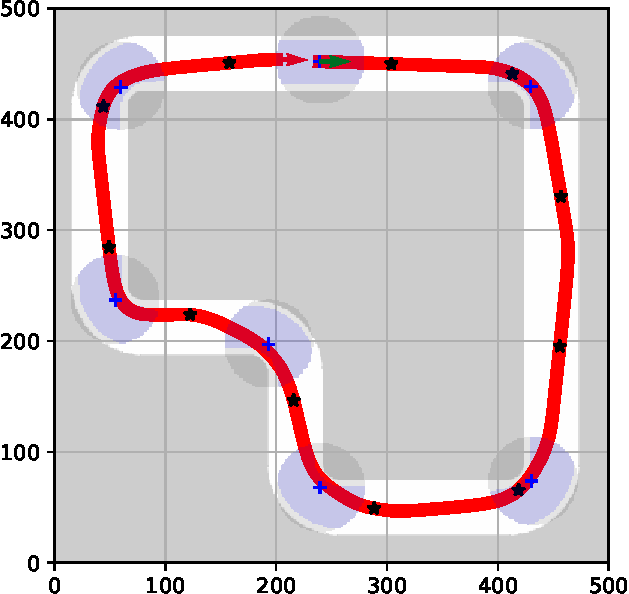
\includegraphics[width=\textwidth]{../img/experiments/simple-sehs-trajectory}
		\end{subfigure}
		\hfill
		\begin{subfigure}[t]{0.45\textwidth}
			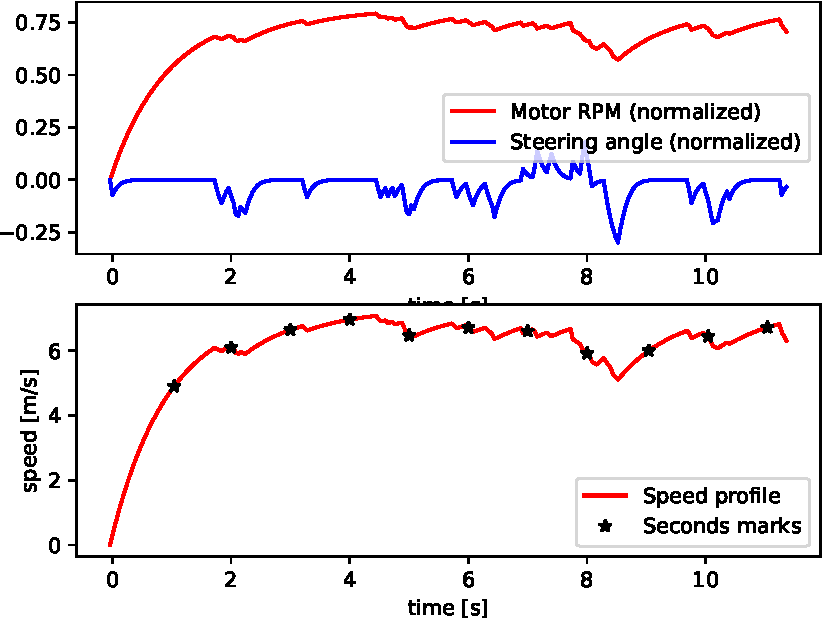
\includegraphics[width=\textwidth]{../img/experiments/simple-sehs-actuators}
		\end{subfigure}
		\caption{Soultion found by SEHS in \SI{449.20}{\milli\second}}
		\label{fig:simple-sehs}
	\end{subfigure}

	\vspace{0.75cm}

	\begin{subfigure}[t]{\textwidth}
		\centering
		\begin{tabular}{r r r r r r r r}%
			\toprule
                Actions & Grid cell size & RPM levels & Heading angle sectors & Opened & Expanded & Search time & Distance & Lap time \\
            \midrule
                \num{44} & \num{1.80} & \num{20} & \num{18} & \bftab \num{78401} & \bftab \SI{236.20}{\milli\second} & \SI{69.75}{\meter} & \SI{20.88}{\second} \\
                \num{84} & \num{1.44} & \num{40} & \num{36} & \num{807771} & \SI{1926.50}{\milli\second} & \SI{67.91}{\meter} & \SI{19.92}{\second} \\
			\bottomrule
		\end{tabular}
		\caption{Hybrid A* results}
		\label{table:simple-hybrid_astar}
    \end{subfigure}
    
    \begin{subfigure}[t]{\textwidth}
		\centering
		\begin{tabular}{r r r r r r r r}%
            \toprule
                Actions & Circles & RPM levels & Heading angle sectors & Opened & Expanded & Search time & Distance & Lap time \\
            \midrule
                \num{44} & \num{134} & \num{20} & \num{18} & \num{129796} & \SI{449.20}{\milli\second} & \SI{71.82}{\meter} & \SI{21.64}{\second} \\
                \num{88} & \num{134} & \num{40} & \num{52} & \num{1443863} & \SI{4204.30}{\milli\second} & \SI{67.76}{\meter} & \bftab \SI{19.76}{\second} \\
			\bottomrule
		\end{tabular}
		\caption{SEHS results}
		\label{table:simple-sehs}
	\end{subfigure}
	
	\vspace{0.75cm}

	\caption{Circuit ``Simple''}
	\label{fig:simple}
\end{figure}

\begin{figure}[!tbp]%
	\centering

	\begin{subfigure}[t]{\textwidth}
		\begin{subfigure}[t]{0.45\textwidth}
			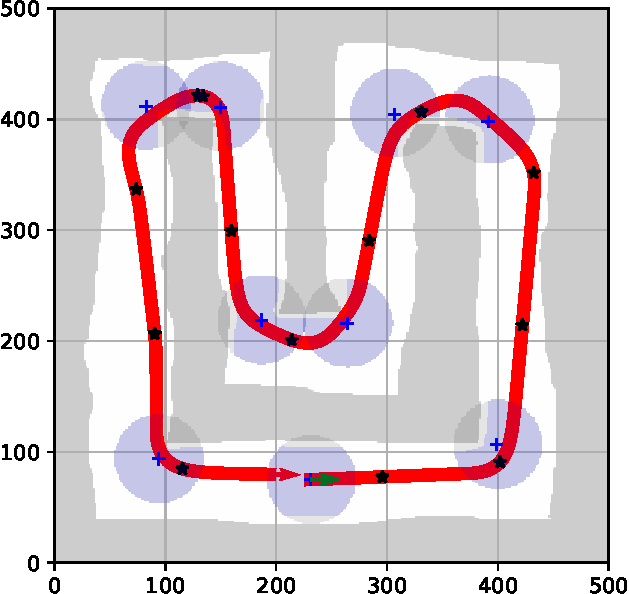
\includegraphics[width=\textwidth]{../img/experiments/u-hybrid_astar-trajectory}
		\end{subfigure}
		\hfill
		\begin{subfigure}[t]{0.45\textwidth}
			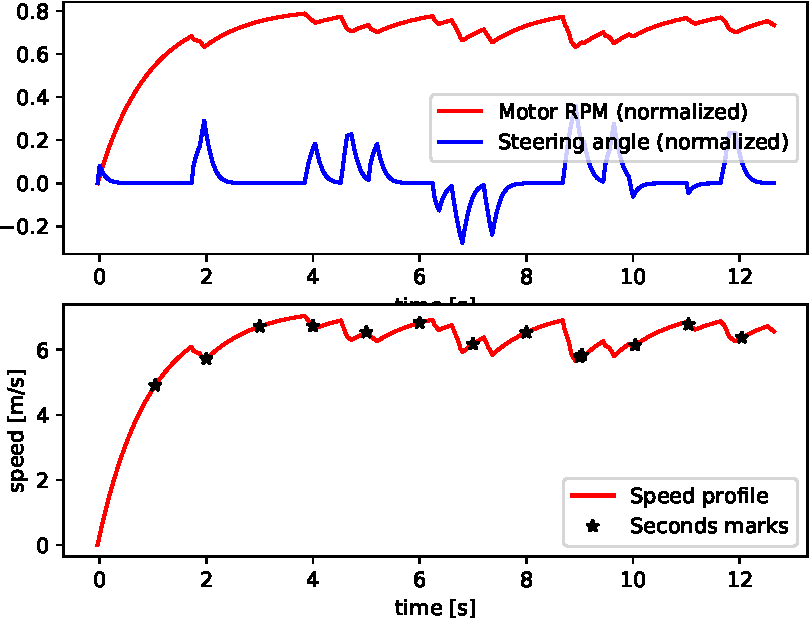
\includegraphics[width=\textwidth]{../img/experiments/u-hybrid_astar-actuators}
		\end{subfigure}	
		\caption{Solution found by Hybrid A* in \SI{440.10}{\milli\second}}
		\label{fig:u-hybrid_astar}
	\end{subfigure}

	\vspace{0.75cm}

	\begin{subfigure}[t]{\textwidth}
		\begin{subfigure}[t]{0.45\textwidth}
			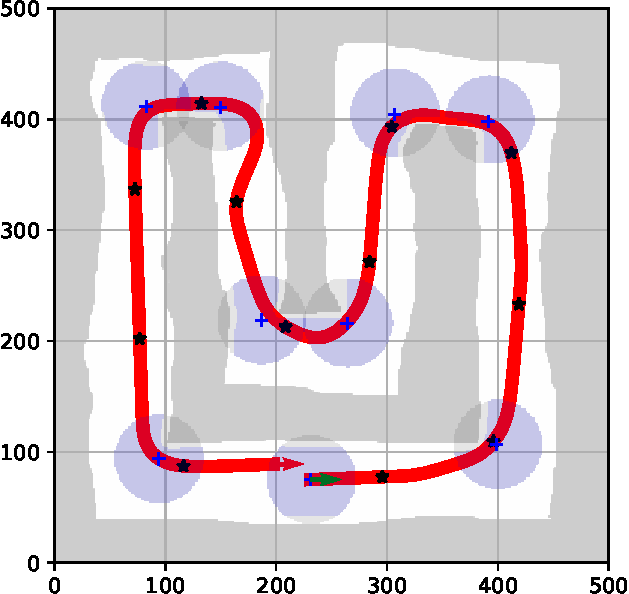
\includegraphics[width=\textwidth]{../img/experiments/u-sehs-trajectory}
		\end{subfigure}
		\hfill
		\begin{subfigure}[t]{0.45\textwidth}
			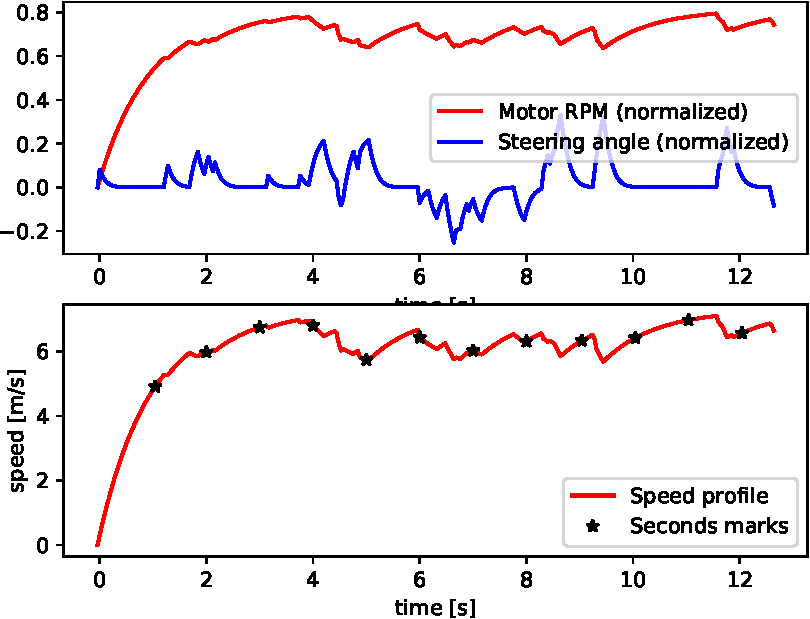
\includegraphics[width=\textwidth]{../img/experiments/u-sehs-actuators}
		\end{subfigure}
		\caption{Solution found by SEHS in \SI{533.60}{\milli\second}}
		\label{fig:u-sehs}
	\end{subfigure}
	
	\vspace{0.75cm}
	
	\begin{subfigure}[t]{\textwidth}
		\centering
		\begin{tabular}{r r r r r r r r}%
        \toprule
            Actions & Grid cell size & RPM levels & Heading angle sectors & Opened & Expanded & Search time & Distance & Lap time \\
        \midrule
            \num{44} & \num{1.80} & \num{20} & \num{18} & \bftab \num{145240} & \bftab \SI{440.10}{\milli\second} & \SI{73.18}{\meter} & \SI{23.08}{\second} \\
            \num{84} & \num{1.44} & \num{40} & \num{36} & \num{1442255} & \SI{3667.90}{\milli\second} & \SI{71.11}{\meter} & \SI{21.84}{\second} \\
		\bottomrule
	\end{tabular}
	\caption{Hybrid A*:}
	\label{table:u-hybrid_astar}
    \end{subfigure}

	\begin{subfigure}[t]{\textwidth}
		\centering
		\begin{tabular}{r r r r r r r r}%
		\toprule
            Actions & Circles & RPM levels & Heading angle sectors & Opened & Expanded & Search time & Distance & Lap time \\
        \midrule
            \num{44} & \num{123} & \num{20} & \num{18} & \num{147605} & \SI{533.60}{\milli\second} & \SI{74.67}{\meter} & \SI{23.64}{\second} \\
            \num{44} & \num{123} & \num{40} & \num{52} & \num{829326} & \SI{2289.80}{\milli\second} & \SI{69.97}{\meter} & \bftab \SI{21.60}{\second} \\
		\bottomrule
	\end{tabular}
	\caption{SEHS:}
	\label{table:u-sehs}
	\end{subfigure}
	
	\vspace{0.75cm}
	
	\caption{Circuit ``U''}
	\label{fig:u}
\end{figure}

\begin{figure}[!tbp]%
	\centering

	\begin{subfigure}[t]{\textwidth}
		\begin{subfigure}[t]{0.45\textwidth}
			\includegraphics[width=\textwidth]{../img/experiments/race_track-hybrid_astar-trajectory}
		\end{subfigure}
		\hfill
		\begin{subfigure}[t]{0.45\textwidth}
			\includegraphics[width=\textwidth]{../img/experiments/race_track-hybrid_astar-actuators}
		\end{subfigure}	
		\caption{Solution found by Hybrid A* in \SI{570.30}{\milli\second}}
		\label{fig:race_track-hybrid_astar}
	\end{subfigure}

	\vspace{0.75cm}

	\begin{subfigure}[t]{\textwidth}
		\begin{subfigure}[t]{0.45\textwidth}
			\includegraphics[width=\textwidth]{../img/experiments/race_track-sehs-trajectory}
		\end{subfigure}
		\hfill
		\begin{subfigure}[t]{0.45\textwidth}
			\includegraphics[width=\textwidth]{../img/experiments/race_track-sehs-actuators}
		\end{subfigure}
		\caption{Solution found by SEHS in \SI{598.10}{\milli\second}}
		\label{fig:race_track-sehs}
	\end{subfigure}
	
	\vspace{0.75cm}
	
	\begin{subfigure}[t]{\textwidth}
		\centering
		\begin{tabular}{r r r r r r r r}%
		\toprule
            Actions & Grid cell size & RPM levels & Heading angle sectors & Opened & Expanded & Search time & Distance & Lap time \\
        \midrule
            \num{44} & \num{1.80} & \num{20} & \num{36} & \num{195755} & \bftab \SI{570.30}{\milli\second} & \SI{85.92}{\meter} & \SI{26.64}{\second} \\
            \num{84} & \num{1.80} & \num{80} & \num{36} & \num{1450767} & \SI{2749.70}{\milli\second} & \SI{82.33}{\meter} & \SI{25.48}{\second} \\
		\bottomrule
	\end{tabular}
	\caption{Hybrid A* peformed worse when compared to SEHS for this track.}
	\label{table:race_track-hybrid_astar}
    \end{subfigure}

	\begin{subfigure}[t]{\textwidth}
		\centering
		\begin{tabular}{r r r r r r r r}%
		\toprule
            Actions & Circles & RPM levels & Heading angle sectors & Opened & Expanded & Search time & Distance & Lap time \\
        \midrule
            \num{44} & \num{164} & \num{20} & \num{18} & \bftab \num{169002} & \SI{598.10}{\milli\second} & \SI{82.66}{\meter} & \SI{25.52}{\second} \\
            \num{124} & \num{164} & \num{20} & \num{52} & \num{1277382} & \SI{4809.20}{\milli\second} & \SI{81.46}{\meter} & \bftab \SI{25.04}{\second} \\
		\bottomrule
	\end{tabular}
	\caption{The solution found by the fastest lap time. Of the two solutions with the lowest computation time, the solution found by SEHS has a significantly better lap time.}
	\label{table:race_track-sehs}
	\end{subfigure}
	
	\vspace{0.75cm}
	
	\caption{Circuit ``Race Track''}
	\label{fig:u}
\end{figure}

\begin{figure}[!tbp]%
	\centering
		
	\begin{subfigure}[t]{\textwidth}
		\begin{subfigure}[t]{0.45\textwidth}
			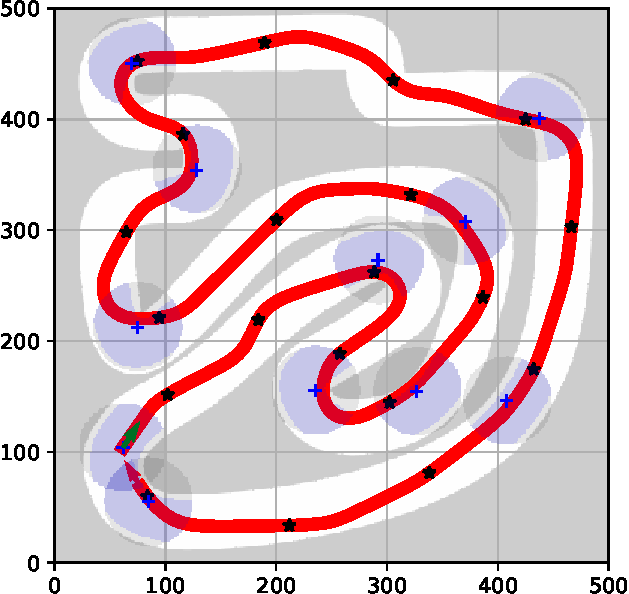
\includegraphics[width=\textwidth]{../img/experiments/zurich-hybrid_astar-trajectory}
		\end{subfigure}
		\hfill
		\begin{subfigure}[t]{0.45\textwidth}
			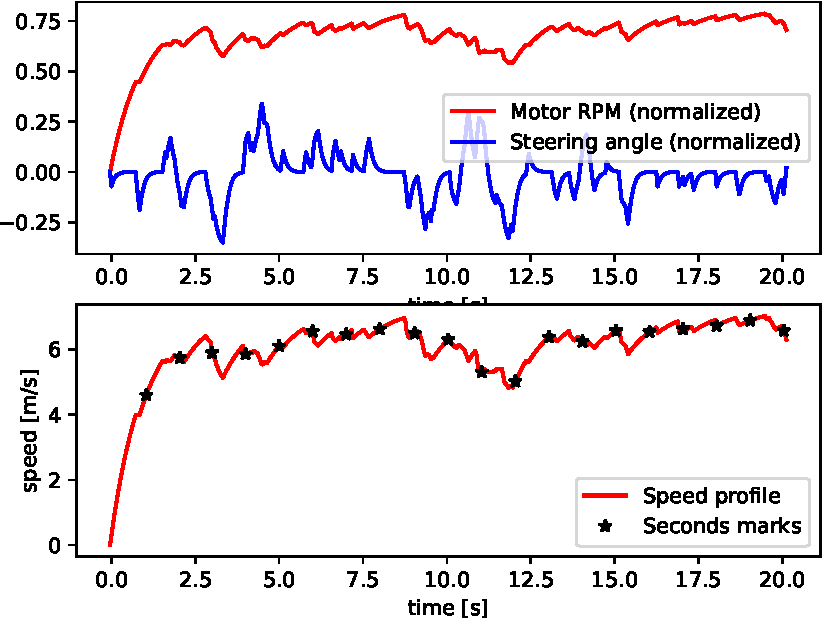
\includegraphics[width=\textwidth]{../img/experiments/zurich-hybrid_astar-actuators}
		\end{subfigure}
		\caption{Solution found by Hybrid A*}
		\label{fig:zurich-hybrid_astar}
	\end{subfigure}

	\vspace{0.75cm}
	
	\begin{subfigure}[t]{\textwidth}
		\centering
		\begin{tabular}{r r r r r r r r}%
            \toprule
                Actions & Grid cell size & RPM levels & Heading angle sectors & Opened & Expanded & Search time & Distance & Lap time \\
			\midrule
                \num{44} & \num{1.80} & \num{40} & \num{36} & \num{488873} & \SI{1041.10}{\milli\second} & \SI{123.67}{\meter} & \SI{41.28}{\second} \\
                \num{88} & \num{1.80} & \num{80} & \num{36} & \num{1922591} & \SI{3811.00}{\milli\second} & \SI{120.09}{\meter} & \SI{38.52}{\second} \\
			\bottomrule
		\end{tabular}
		\caption{Hybrid A* was the only algorithm of the two which found a solution. The SEHS algorithm did not find any solution for any combination of the parameters.}
		\label{table:zurich-hybrid_astar}
    \end{subfigure}
	
	\vspace{0.75cm}

	\caption{Circuit ``Zurich''}
	\label{fig:zurich}
\end{figure}

\section{Autonomous Race}

To further test the algorithms, we implemented the complete Artificial Racing Agent on top of the \gls{ROS} and we built a custom hardware inspired by the F1/10 platform. The details of the implementation are described in the appendixes Experimental Vehicle (Appendix~\ref{chapter:hardware}) and Technical Documentation (Appendix~\ref{chapter:technical_documentation}).

In the following experiments, we tried to test the racing capabilities of the vehicle. The vehicle was given a complete map of the circuit at the beginning of the race. The goal was to go around the circuit repeatedly without colliding with walls and obstacles and reaching the best lap times as possible.

The agent repeatedly triggers the \gls{SEHS} based trajectory planning algorithm from the latest known state of the vehicle with the latest known state of the map with the obstacles marked in it through the current list of waypoints. At the same time, the vehicle is already driving and following the last published trajectory. Once the planning algorithm comes up with a new plan, it replaces the old plan and it can start planning again with the latest known state.

\subsection{Testing Criteria}
For the planning algorithm to be viable, it must calculate the trajectory in a short period of time before the vehicle physically moves to the end of the previous trajectory. We were also interested in the safety of the planned trajectory and the distance the vehicle keeps from the obstacles while following the trajectory. Finally, our goal is to achieve fast lap times and we are interested in the maximum speed our vehicle can achieve while driving safely.

\subsection{Real World Testing}

\begin{figure}
	\label{fig:real-world-testing-still}
	\centering
	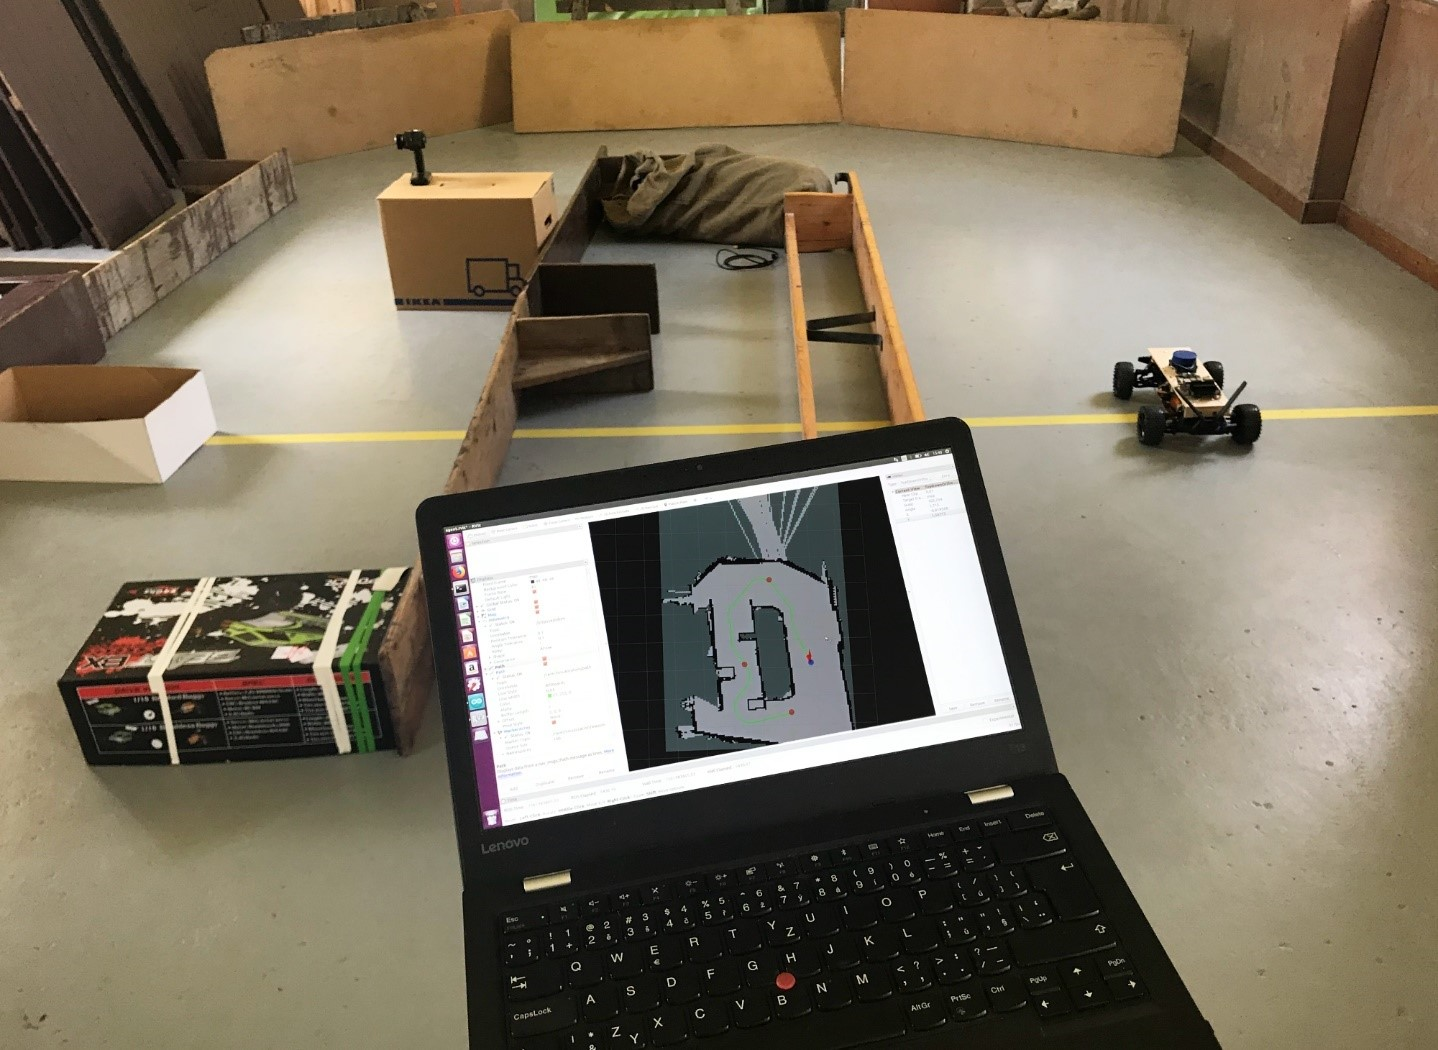
\includegraphics[width=\textwidth]{../img/experiments/real-world-still.jpg}
	\caption{The planning algorithm finds a trajectory from the last known state of the vehicle through the waypoints ahead of it while avoiding the obstacles marked in the map.}
\end{figure}


Initially, we wanted to perform tests outdoors on an asphalt plane, but it proved problematic because of surface curvature and unstable weather conditions. Another unexpected problem we had to solve was a problem with the \gls*{LIDAR} unit. It performed very unreliably in direct sunlight. In the end, we tested our vehicle indoors in a rectangular gym \SI{10}{\meter} long and \SI{6}{\meter} wide with concrete surface which was available to us for several days. We built several versions of an obstacle course using gym equipment and from cardboard boxes. One such circuit is shown in Figure~\ref{fig:real-world-testing-still}.

The experiment consisted of two phases. First, we built a 2D map from the data coming from the \gls*{LIDAR} as the vehicle drove around the track using a remote controller. Using this map, we assembled a configuration file describing the racing circuit. Next, we started all the \gls{ROS} nodes for vehicle state monitoring, circuit progress monitoring, trajectory planning, and trajectory following. Once the planning algorithm produces the first trajectory, the vehicle would start following it. We were closely monitoring the movement of the vehicle visually and using telemetry data on a laptop through the \texttt{Rviz} program\footnote{\url{http://wiki.ros.org/rviz}}. We were always ready to take control of the vehicle using the remote control to prevent damage to the vehicle and to its surroundings. Any input from the controller would cancel the autonomous mode and switch the vehicle into a remote-control mode. The vehicle then stayed in this mode until a button on the vehicle was physically pressed.

We struggled with unreliable odometry for several days. We tested several different localization libraries, adjusted data collected from the sensors, and tweaked the parameters of the libraries until we were able to get usable odometry data at least at low speeds. At higher speeds, the vehicle would quickly lose track of its actual position and orientation on the map and it would collide with a wall or with an obstacle.

By the end of the testing, the vehicle was able to reliably circle around the track without hitting obstacles and without the odometry significantly diverging from the actual state of the vehicle. The car repeatedly completed a circuit which was approximately 20 meters long in 15 seconds at a steady speed of \SI{1.3}{\meter\per\second}~(\SI{4.68}{\kilo\meter\per\hour}) which corresponds to a speed of \SI{46.8}{\kilo\meter\per\hour} of a full-size vehicle. At this speed, the limitations of the kinematic model do not manifest, and the vehicle had no issues undershooting or overshooting turns. A photo from this test is shown in Figure~\ref{fig:real-world-testing-driving} and a video recording of this experiment is available in the attachment of this thesis \todo{Add the path to the file in a footnote}.

\begin{figure}
	\label{fig:real-world-testing-driving}
	\centering
	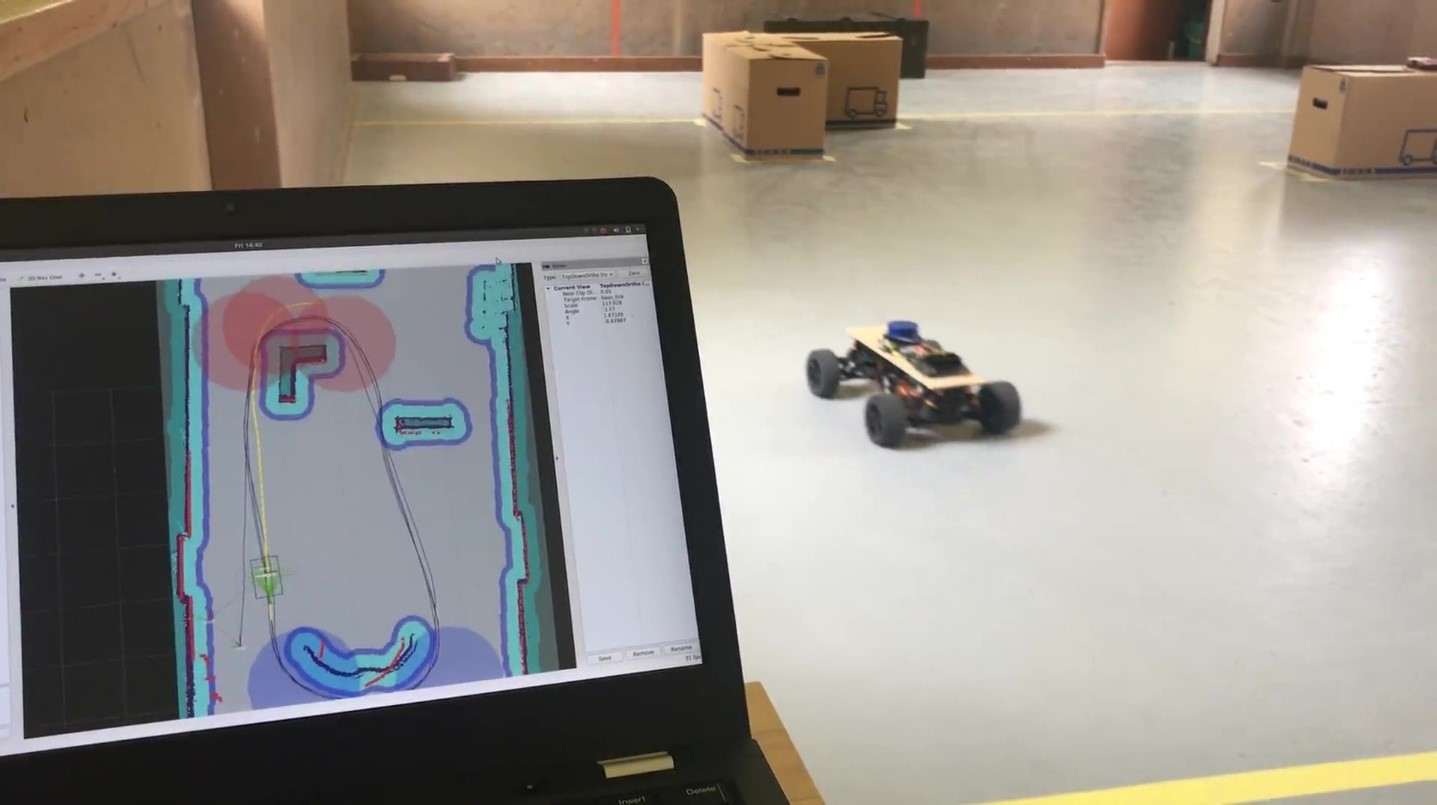
\includegraphics[width=\textwidth]{../img/experiments/real-world-driving.jpg}
	\caption{The vehicle is slowly driving along a circuit in a gym. The telemetry from the vehicle is monitored on a notebook connected to the vehicle over Wi-Fi.}
\end{figure}

The trajectory planning algorithm performed well even with just the low-powered ARM processor and the vehicle had never reached the end of the planned trajectory before a new extended trajectory was published. The \gls{DWA} algorithm kept the vehicle on the track and avoided all crates along the circuit.

Although the robot was able to navigate autonomously without collisions, the speeds we were able to reach were too low and did not reach a speed at which we would start seeing any effects of high speed maneuvers, such as wheel slipping and skidding and overshooting corners. We were also unable to test evasion of dynamic obstacles because the obstacle detection library produced too many ghost obstacles from our noisy and low-frequency \gls*{LIDAR} scans.

\subsection{Simulator}
Due to the hardware issues we ran into and due to other factors, which did not allow further improvements and testing of the vehicle during the spring of 2020, we conducted further experiments only with the Gazebo simulator \cite{gazebo} configured for the F1/10 platform \cite{varundev_ros_19}. This change gave us the opportunity to test the algorithm with perfect odometry, but with the same interface between the algorithm and the simulated actuators of the virtual vehicle. To adapt the algorithm for the simulator, we had to modify our steering servo and motor models. We tweaked the parameters of our models to predict the behavior of the simulated vehicle as closely as possible.

The F1/10 simulator repository\footnote{\url{https://github.com/f1tenth-dev/simulator}} contains a 3D map with several different types of corners and it is shown in Figure~\ref{fig:gazebo-track}. Especially the middle part which consists of a series of left-hand turn followed by a right-hand hairpin turn presents a challenge where the car must slow down to avoid collision while keeping as much speed as possible to still reach a good lap time. We ran the full-circuit planning for the modified vehicle model and for this track. The planned trajectories are shown in Figure~\ref{fig:sim-race_track}.

For this experiment, we turned off obstacle detection and we focused only on the lap times in a track without any obstacles. We tried three different algorithms and for each of them, we let it run for up to 10 consecutive laps. We ran each algorithm three times and we used the run in which it was able to complete all of the 10 laps and in which it reached the best average lap time.

\begin{figure}
	\label{fig:gazebo-track}
	\centering
	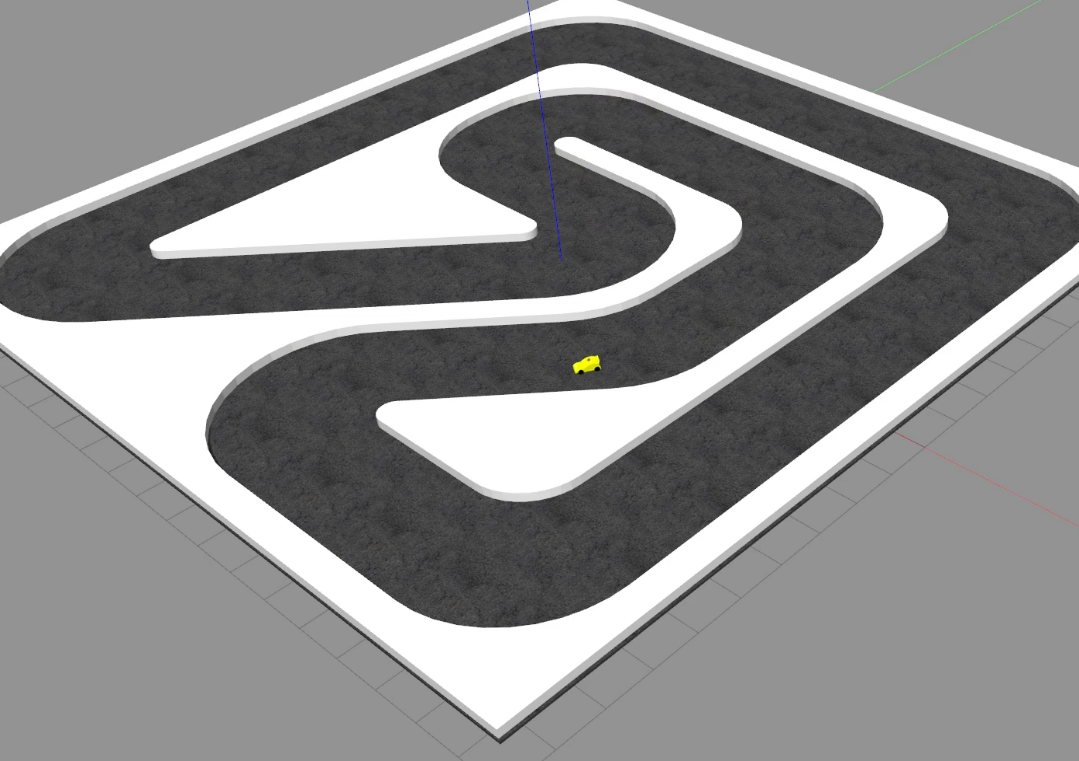
\includegraphics[width=\textwidth]{../img/experiments/gazebo-track.png}
	\caption{The testing track contains several long straights and several challenging turns. The Gazebo simulator allows us to monitor and modify the 3D scene.}
\end{figure}

\begin{figure}
	\label{fig:rviz-planned-track}
	\centering
	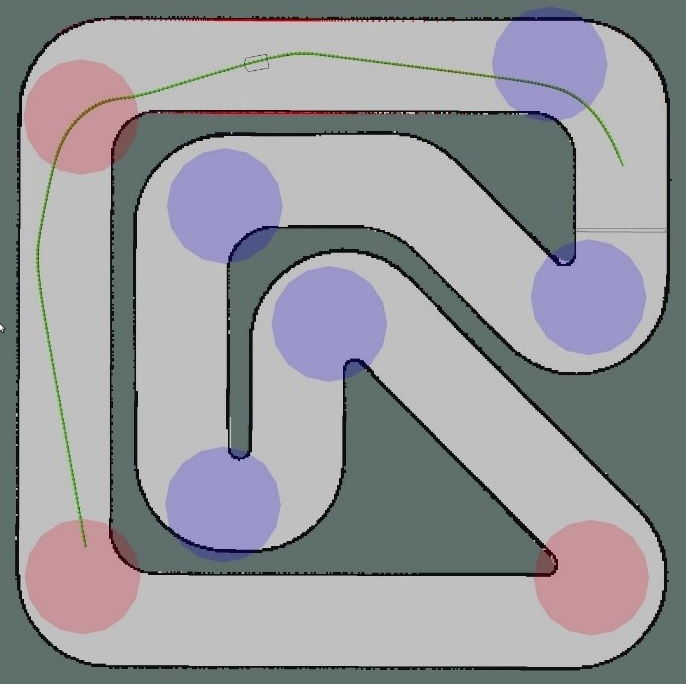
\includegraphics[width=\textwidth]{../img/experiments/rviz-planned-track.jpg}
	\caption{This figure captures a planned trajectory and a vehicle on the testing track as it is shown in Rviz. The circles represent the positions of the corners detected by the track analysis algorithm. The circles marked in red are the next three corners ahead of the vehicle. The mostly green line represents the last planned trajectory. Green parts of the trajectory show where the vehicle is expected to drive fast and red parts would show where the vehicle should slow down.}
\end{figure}

\paragraph{Reference Implementation}
The F1/10 Simulator repository contains a reference implementation of the Pure Pursuit algorithm which follows a fixed spline path divided sectors marked as “unrestricted”, “caution”, and “brake”, which tell the vehicle how to adjust its speed. We used this implementation as a baseline and we will compare our results against this implementation. This algorithm cannot react to any unexpected obstacles.

\paragraph{\gls{SEHS} and Pure Pursuit}
The first trajectory following algorithm we tested was the combination of the \gls*{SEHS} planning algorithm and the Pure Pursuit controller. We tested different values of the lookahead distance, and we settled on an adaptive look ahead distance linearly proportional to the speed of the vehicle. The lookahead was set to \SI{0.5}{\meter} for a stopped vehicle and \SI{2.0}{\meter} for the theoretical top speed. This algorithm has no mechanism of avoiding unexpected obstacles which were not considered by the planning algorithm and pure pursuit would blindly hit an obstacle if the reference trajectory went through it.

\paragraph{\gls{SEHS} and \gls{DWA}}
The other controller we tested was the \gls{DWA} algorithm. This algorithm has several parameters which we tuned until we reached satisfying results. First parameter is the prediction horizon which determines for how long we predict the movement of the vehicle from the current measured state with a single examined action. Short prediction horizon does not give enough room to reveal differences between all the applicable actions and a long prediction horizon is unrealistic, because we change the action several times per second and it also eliminates many actions, because fixating one action for too long would likely lead to a collision. We achieved best results by setting the prediction horizon to \SI{0.3}{\second}.

The other parameters are the weights we assign to the error of the position of the vehicle, the error of its heading angle, the error of the speed of the vehicle, and the proximity to the obstacles ahead of the vehicle and nearby obstacles. In the end, the highest weight was assigned to the distance from obstacles and the second largest to the position error.

Thanks to the fact the obstacle proximity factor, which is considered by the \gls*{DWA} algorithm, it can steer the vehicle around obstacles which are detected using the \gls*{LIDAR} scans. We tested this by placing cubes and cylinders on the track in the Gazebo application. We tried placing the obstacles in several different ways. We tried blocking the apexes of a corner and forcing the vehicle to go along the outer wall. We also placed two boxes along each side of the track and forced the vehicle to go through a narrow gap in the middle. The third experiment with obstacles consisted of placing three boxes one after each other at sides of the track in an alternating pattern to block passage in a straight line. The success of avoidance was significantly impacted by the prediction horizon parameter. When this parameter was too short, the vehicle would notice the obstacle too late and it would not have enough room to avoid it and it would collide.

The planning algorithm could fail when the occasional misalignment of the \gls*{LIDAR} scans with the map caused ghost obstacles around the actual obstacles and around the walls being marked in the occupancy grid. Especially in the scenario with a narrow passage between two boxes, the track would seem completely blocked to the planning algorithm and it would not be able to produce a reference trajectory. We managed to reduce this effect by tuning the parameters of the obstacle detection library, but we were not able to eliminate this problem.

\paragraph{Results}

The simulated vehicle follows this trajectory almost flawlessly and during a test run of 10 consecutive laps it reached an average lap time of \SI{26.410}{\second} with top speed reaching \SI{4.08}{\meter\per\second} and the best lap time in this run was \SI{25.911}{\second}. For detailed statistics of lap times and speeds achieved by this algorithm, see Table~\ref{tbl:reference-impl}.

The trajectory analysis algorithm correctly detects eight corners of the circuit. We set the planning algorithm to plan for the next 3 corners ahead of it. The planning time on the desktop computer ranged between \SI{60}{\milli\second} and \SI{100}{\milli\second} depending on the initial state and on the length and complexity of the circuit segment ahead of the vehicle.

In our test, the \gls*{DWA} algorithm was achieve an average lap time of \SI{26.239}{\s} with the best lap time of \SI{23.855}{\s} and reaching a top speed of \SI{4.08}{\meter\per\second}. The Pure Pursuit algorithm achieved an average lap time of \SI{28.319}{\s} with the best lap time of \SI{26.908}{\s} and reaching a top speed of \SI{4.00}{\meter\per\second}. The detailed results of the experiment can be seen in Table~\ref{tbl:dwa} and Table~\ref{tbl:pure-pursuit}.

\todo[inline]{Compare this to the pre-planned times.}

\begin{table}
	\centering
	\label{tbl:reference-impl}
	\begin{tabular}{c c c c c}
		\toprule
		& Lap time       & Distance traveled  & Average speed             & Maximum speed             \\
		& [\si{\second}] & [\si{\meter}]      & [\si{\meter\per\second}]  & [\si{\meter\per\second}]  \\
		\midrule
		1. & 27.876 & 84.72 & 3.25 & 4.06 \\
		2. & 26.208 & 87.07 & 3.37 & 4.08 \\
		3. & 26.381 & 86.91 & 3.38 & 4.07 \\
		4. & 26.279 & 86.75 & 3.36 & 4.06 \\
		5. & 26.484 & 87.00 & 3.35 & 4.05 \\
		6. & 26.172 & 86.96 & 3.37 & 4.07 \\
		7. & 26.366 & 87.03 & 3.37 & 4.07 \\
		8. & 26.227 & 86.54 & 3.37 & 4.08 \\
		9. & \textbf{25.911} & \textbf{85.83} & \textbf{3.37} & \textbf{4.05} \\
		10. & 26.199 & 86.39 & 3.36 & 4.06 \\
	
		\bottomrule
	\end{tabular}
	\caption{The results of ten consecutive laps achieved with the reference implementation of the Pure Pursuit algorithm following a predefined curve. This implementation was taken from the F1/10 Simulator GitHub repository.}
\end{table}

\begin{table}
	\centering
	\label{tbl:dwa}
	\begin{tabular}{c c c c c}
		\toprule
		    & Lap time       & Distance traveled  & Average speed             & Maximum speed             \\
		    & [\si{\second}] & [\si{\meter}]      & [\si{\meter\per\second}]  & [\si{\meter\per\second}]  \\
		\midrule
		1. & 33.422 & 88.45 & 2.96 & 3.83 \\
		2. & \textbf{23.855} & \textbf{86.83} & \textbf{3.64} & \textbf{4.08} \\
		3. & 24.222 & 87.48 & 3.61 & 4.02 \\
		4. & 25.065 & 86.63 & 3.46 & 3.96 \\
		5. & 26.248 & 90.11 & 3.43 & 3.90 \\
		6. & 25.876 & 89.05 & 3.45 & 3.90 \\
		7. & 25.428 & 87.21 & 3.44 & 3.89 \\
		8. & 27.576 & 88.57 & 3.23 & 3.88 \\
		9. & 25.779 & 85.47 & 3.32 & 3.79 \\
		10.& 24.922 & 86.62 & 3.47 & 3.97 \\
		\bottomrule
	\end{tabular}
	\caption{The results of ten consecutive laps achieved with the combination of the SEHS and DWA algorithms in the Gazebo simulator.}
\end{table}

\begin{table}
	\centering
	\label{tbl:pure-pursuit}
	\begin{tabular}{c c c c c}
		\toprule
		& Lap time       & Distance traveled  & Average speed             & Maximum speed             \\
		& [\si{\second}] & [\si{\meter}]      & [\si{\meter\per\second}]  & [\si{\meter\per\second}]  \\
		\midrule
		1.  & 32.200 & 84.66 & 2.88 & 3.72 \\
		2.  & 28.404 & 88.05 & 3.13 & 3.84 \\
		3.  & 27.612 & 87.83 & 3.18 & 3.85 \\
		4.  & 27.042 & 86.38 & 3.21 & 3.80 \\
		5.  & 27.645 & 86.82 & 3.15 & 3.75 \\
		6.  & 29.277 & 87.35 & 3.04 & 3.72 \\
		7.  & \textbf{26.908} & \textbf{88.09} & \textbf{3.27} & \textbf{4.00} \\
		8.  & 27.904 & 87.72 & 3.15 & 3.73 \\
		9.  & 27.669 & 87.64 & 3.17 & 3.87 \\
		10. & 28.528 & 88.82 & 3.13 & 3.74 \\

		\bottomrule
	\end{tabular}
	\caption{The results of ten consecutive laps achieved with the combination of the SEHS and Pure Pursuit algorithms in the Gazebo simulator.}
\end{table}

\todo[inline]{Add also the results achieved with the Hybrid A* algorithm.}

\todo[inline]{Add also the lines the different algorithms took.}

The \gls{SEHS} algorithm proved to be fast enough and to produce reasonable reference trajectories even at the higher speeds which we achieved in the simulator. The algorithm was able to produce new plans at a rate of up to \SI{15}{\hertz}. The only problem we were experiencing was a drop of the re-planning frequency in the middle section of the track. The algorithm was sometimes not able to find a trajectory in the series of a tight left run followed-up with a hairpin turn. Each of the trajectories the algorithm tested resulted in a collision with the boundary of the track. Most of the time, the car would slow down enough that the algorithm could find a trajectory to the next waypoint, but sometimes the car would keep following the trajectory to its end and then it would not have anything to follow. The Pure Pursuit algorithm would immediately crash into the road boundary and get stuck. The \gls*{DWA} algorithm on the other hand can follow further guided just by obstacle avoidance. Once the vehicle reaches the apex of the hairpin turn, the planning algorithm is able to find a collision-free trajectory to the waypoints ahead of the vehicle and it can continue the race with only a small worsening of the lap time.

Both the Pure Pursuit and the \gls*{DWA} algorithms worked well in the simulator after their parameters were tuned. The Pure Pursuit algorithm performed slightly worse than the reference implementation. The \gls*{DWA} algorithm on the other hand reached the fastest lap times of the three algorithms on average and it also managed to reach the fastest lap time of \SI{23.855}{\second}. On top of that, it was more robust thanks to the ability to continue driving forward even without a guiding trajectory and it is therefore the winner of this race.

\subsection{Obstacle Avoidance}

\todo[inline]{Write this chapter.}
